	El reactor de flujo pistón trabaja en estado estacionario. Esto significa que las propiedades no varían con el tiempo.
	
	En el menú principal, encontramos tres botones dentro del apartado de reactores flujo pistón. Estos tres botones hacen referencia cada a uno a distintas condiciones en las que el reactor flujo pistón puede realizar su operación: reactor flujo pistón isotermo, reactor flujo pistón adiabático y reactor flujo pistón no isotermo y no adiabático.
	
\section{Reactor flujo pistón isotermo}
Si seleccionamos el caso del reactor flujo pistón isotermo, nos aparece una ventana como la que se puede observar en la Figura \ref{fig:ventana_isotermo}.

\begin{figure}[h!]
	\begin{center}
		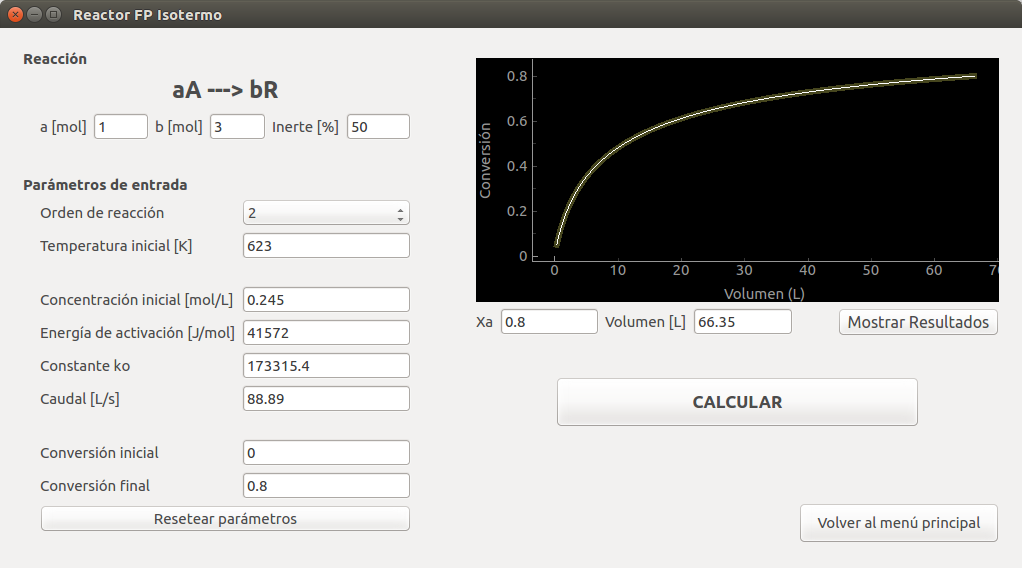
\includegraphics[width=0.85\textwidth]{./imagenes/reactor_fp/isotermo1.png}\caption{Ventana reactor FP isotermo}\label{fig:ventana_isotermo}
	\end{center}
\end{figure}

En la parte superior izquierda, el programa nos indica el tipo de reacción con la que vamos a trabajar y permite modificar el número de reactivos y productos, así como añadir el porcentaje deseado de inerte en la reacción. Una vez que hayamos establecido la reacción deseada, deberemos seleccionar el orden de reacción en el desplegable e introducir todos los parámetros de entrada indicados, prestando especial atención a las unidades en las que se indican que han de ser introducidos.

Cuando tengamos introducidos todos los datos que se indican, podremos obtener el resultado final pulsado sobre el botón \textbf{'CALCULAR'} situado en la parte derecha de la ventana. Inmediatamente después de pulsar sobre dicho botón el programa representará gráficamente el resultado en el gráfico de la parte derecha de la ventana, y se indicará el resultado obtenido, en función de nuestros parámetros de entrada, en las celdas situadas en la parte inferior del gráfico.

Otra de las opciones que pone a nuestra disposición este software es la de observar el gráfico en una ventana independiente ((Figura \ref{fig:ventana_graficas_iso})), pulsando sobre el botón \textbf{'Mostrar Resultados'}. En esta nueva ventana, no solo podremos ver el mismo gráfico descrito anteriormente, sino que además dispondremos de un cursor que nos permitirá ver el resultado en cada punto deseado (antes el resultado dado en las celdas inferiores al gráfico solo mostraba el resultado teniendo en cuenta los parámetros de entrada). En esta nueva ventana también se nos permite exportar el gráfico como una imagen.

\begin{figure}[h!]
	\begin{center}
		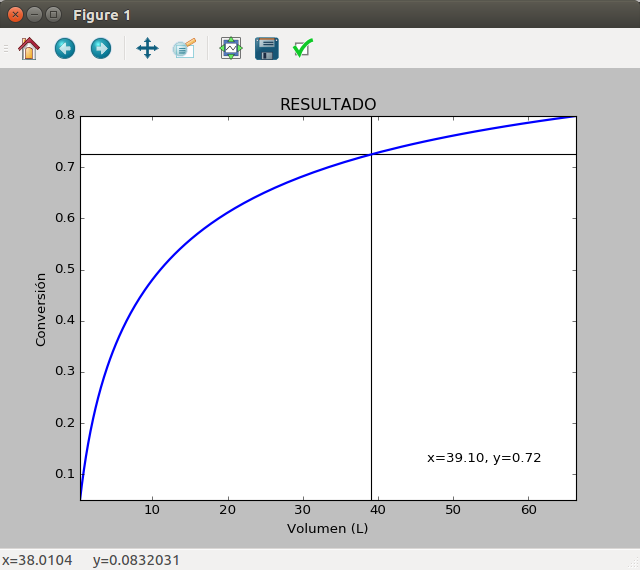
\includegraphics[width=0.85\textwidth]{./imagenes/reactor_fp/isotermo2.png}\caption{Ventana de resultados reactor FP isotermo}\label{fig:ventana_graficas_iso}
	\end{center}
\end{figure}

Finalmente, podemos realizar un borrado de todas las celdas, mediante el botón \textbf{'Resetear parámetros'}, para realizar un nuevo cálculo. Si no deseamos realizar más cálculos y queremos regresar al menú principal, podremos hacerlo pinchando sobre el botón \textbf{'Volver al menú principal'}, situado en la parte inferior derecha de la ventana.


\section{Reactor flujo pistón adiabático}
Seleccionando el reactor flujo pistón adiabático, se nos abrirá una ventana como la mostrada en la Figura \ref{fig:ventana_adiabatico}.

\begin{figure}[h!]
	\begin{center}
		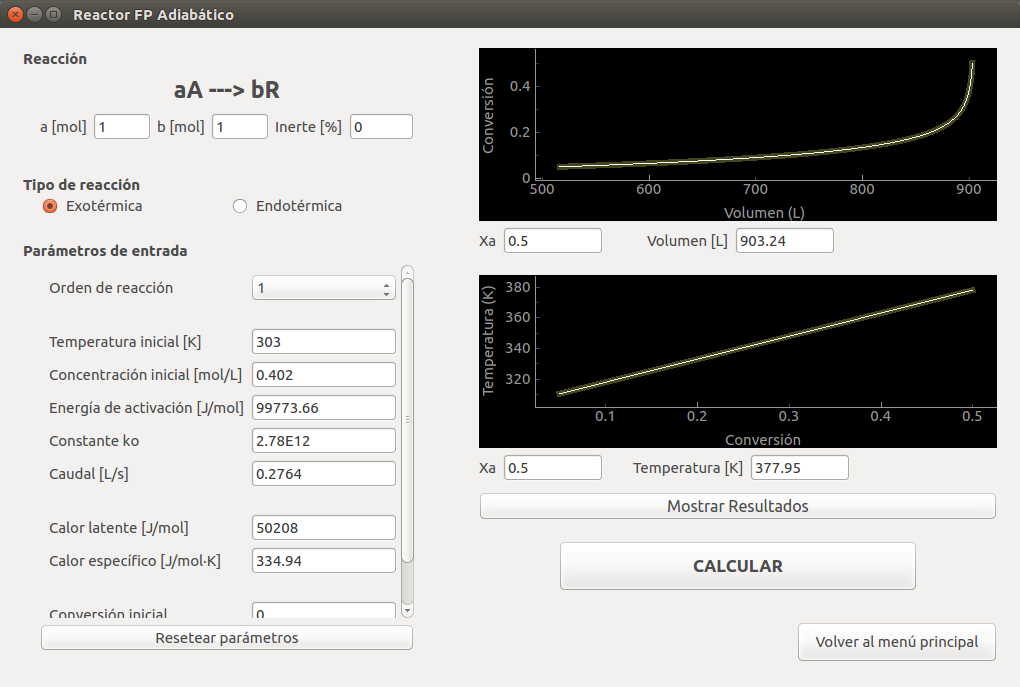
\includegraphics[width=0.85\textwidth]{./imagenes/reactor_fp/adiabatico1.png}\caption{Ventana reactor FP adiabático}\label{fig:ventana_adiabatico}
	\end{center}
\end{figure}

De nuevo, en la parte superior izquierda se nos indica el tipo de reacción con la que vamos a trabajar y se nos permite modificar el número de reactivos y productos, así como añadir el porcentaje deseado de inerte en la reacción. Seguidamente, debido a que estamos trabajando con el caso adiabático, debemos indicar si la reacción será exotérmica o endotérmica. Una vez realizadas estas operaciones, seleccionaremos el orden de reacción en el desplegable y a continuación introduciremos todos los parámetros de entrada indicados, prestando especial atención a las unidades en las que se indican que han de ser introducidos.

Cuando tengamos introducidos todos los datos que se indican, podremos obtener el resultado final pulsando sobre el botón \textbf{'CALCULAR'} situado en la parte derecha de la ventana. Para este reactor, después de pulsar sobre dicho botón, se representarán dos gráficas en lugar de una. Estas gráficas harán referencia al volumen del reactor (gráfico superior) y a la temperatura de la reacción (gráfico inferior). Los resultados numéricos obtenidos, en función de nuestros parámetros de entrada, se mostrarán en las celdas situadas en la parte inferior de cada uno de los gráficos.

Para ver los resultados en una ventana independiente (Figura \ref{fig:ventana_graficas_ad}) bastará con pulsar sobre el botón \textbf{'Mostrar Resultados'}. En esta nueva ventana, como en el caso anterior, dispondremos de un cursor que nos permitirá movernos a través de ambas curvas para ver el resultado del volumen y la temperatura en cada uno de los puntos que deseemos. En esta nueva ventana también se nos permite exportar el gráfico como una imagen.

\begin{figure}[h!]
	\begin{center}
		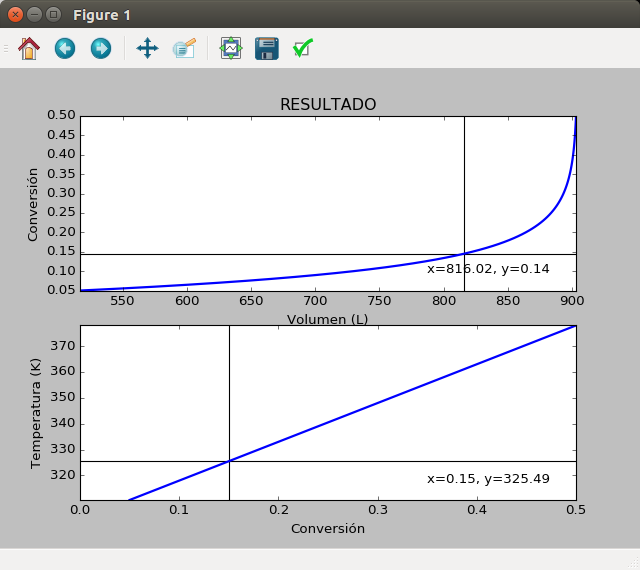
\includegraphics[width=0.85\textwidth]{./imagenes/reactor_fp/adiabatico2.png}\caption{Ventana de resultados reactor FP adiabático}\label{fig:ventana_graficas_ad}
	\end{center}
\end{figure}

Finalmente, podemos realizar un borrado de todas las celdas, mediante el botón \textbf{'Resetear parámetros'}, para realizar un nuevo cálculo. Si no deseamos realizar más cálculos y queremos regresar al menú principal, podremos hacerlo pinchando sobre el botón \textbf{'Volver al menú principal'} de abajo a la derecha de la ventana.


\section{Reactor flujo pistón no adiabático y no isotermo}
Seleccionando el reactor flujo pistón no adiabático y no isotermo, se nos abrirá una ventana como la mostrada en la Figura \ref{fig:ventana_noadi_noiso}.

\begin{figure}[h!]
	\begin{center}
		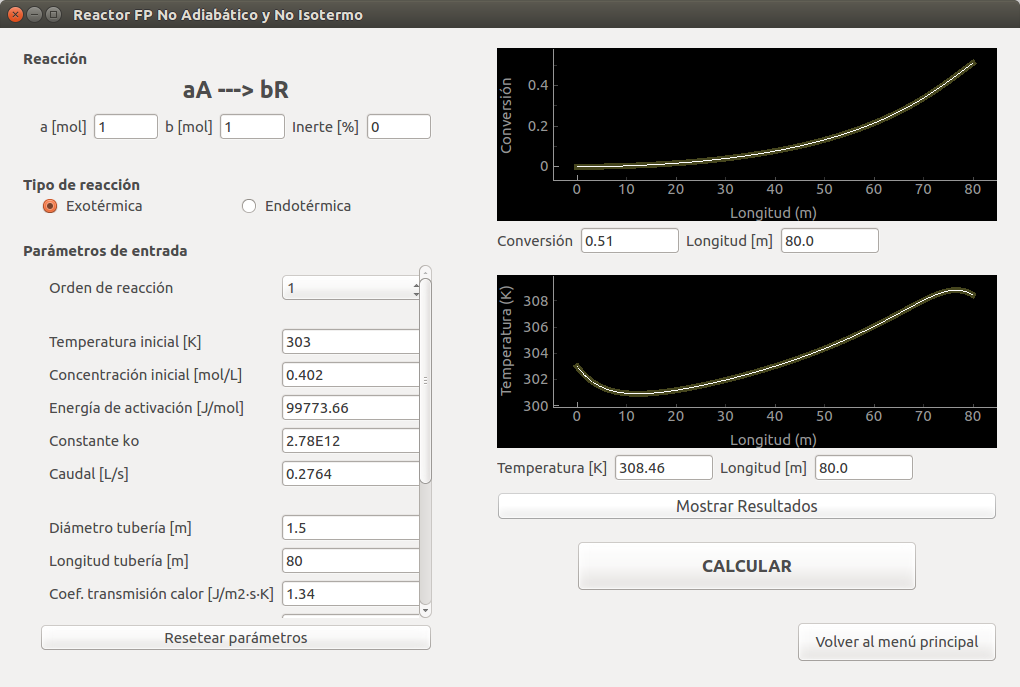
\includegraphics[width=0.85\textwidth]{./imagenes/reactor_fp/no_adi_no_iso1.png}\caption{Ventana reactor FP no adiabático y no isotermo}\label{fig:ventana_noadi_noiso}
	\end{center}
\end{figure}

La estructura de esta ventana es similar a la del caso anterior (reactor flujo pistón adiabático), mostrando en la parte superior izquierda el tipo de reacción con la que vamos a trabajar. Permite modificar el número de reactivos y productos, así como añadir el porcentaje deseado de inerte en la reacción. A continuación, debemos indicar si la reacción será exotérmica o endotérmica. Una vez realizadas estas operaciones, seleccionamos el orden de reacción en el desplegable y procedemos a introducir todos los parámetros de entrada indicados, prestando especial atención a las unidades en las que se indican que han de ser introducidos.

Cuando tengamos introducidos todos los datos, podremos obtener el resultado final pulsado sobre el botón \textbf{'CALCULAR'} situado en la parte derecha de la ventana. Después de pulsar sobre dicho botón, se representarán dos gráficas como ocurría en el caso anterior. Dichas gráficas harán referencia a la conversión que puede lograr el reactor (gráfico superior) y a la temperatura de la reacción (gráfico inferior), ambas en función de la longitud de la tubería. Los resultados numéricos obtenidos, en función de nuestros parámetros de entrada, se mostrarán en las celdas situadas en la parte inferior de cada uno de los gráficos.

\begin{figure}[h!]
	\begin{center}
		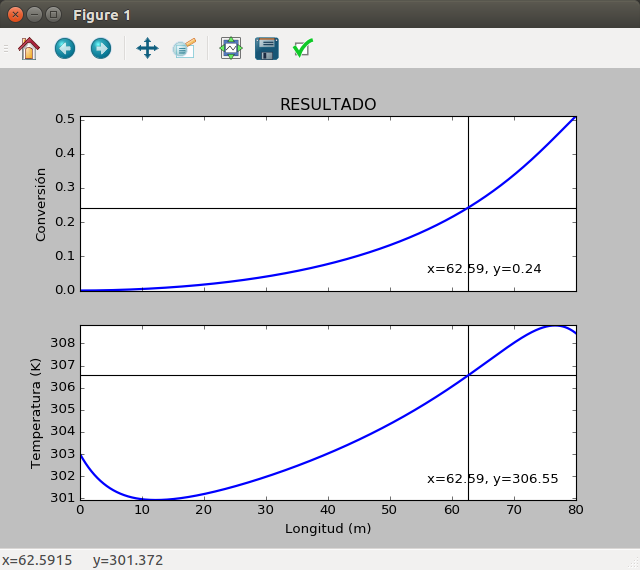
\includegraphics[width=0.85\textwidth]{./imagenes/reactor_fp/no_adi_no_iso2.png}\caption{Ventana de resultados reactor FP no adiabático y no isotermo}\label{fig:ventana_graficas_noadi_noiso}
	\end{center}
\end{figure}

Para ver los resultados en una ventana independiente (Figura \ref{fig:ventana_graficas_noadi_noiso}) bastará con pulsar sobre el botón \textbf{'Mostrar Resultados'}. En esta nueva ventana, como en los casos anteriores, dispondremos de un cursor que nos permitirá movernos a través de ambas curvas para ver el resultado de conversión y temperatura en cada punto concreto. También podremos exportar el gráfico como una imagen.

Finalmente, podemos realizar un borrado de todas las celdas, mediante el botón \textbf{'Resetear parámetros'}, para realizar un nuevo cálculo. Si no deseamos realizar más cálculos y queremos regresar al menú principal, podremos hacerlo pinchando sobre el botón \textbf{'Volver al menú principal'}, situado en la parte inferior derecha de la ventana.